\documentclass[10pt,aspectratio=169]{beamer}
\usefonttheme{professionalfonts}
%\usetheme{Rochester}
%\usetheme{AnnArbor}
\usetheme{Szeged}
\useoutertheme{infolines}
\usecolortheme{dolphin}
\usepackage{graphicx}
% \usepackage[english]{babel}
\usepackage{hyperref}
\usepackage{multicol}
\usepackage{color}
%\usepackage{smartdiagram}


%\definecolor{carmine}{rgb}{0.59, 0.0, 0.09}
\usepackage{amsmath} 

\usepackage{graphicx}
\usepackage{tikz}
\usetikzlibrary{shapes.callouts}
\usepackage{multirow}

\usepackage[utf8]{inputenc}

\usepackage{enumerate}
\usepackage[shortlabels]{enumitem}
\usepackage{amsmath,amsthm,amssymb,amsfonts,mathrsfs,latexsym,stmaryrd}
\usepackage{tcolorbox}

\usepackage{color} 
\usepackage{amssymb, amsmath, amsbsy}
\usepackage{adjustbox,lipsum}
\usepackage{placeins}

\usepackage{textpos}
\usepackage{wrapfig}
\usepackage[spanish, es-tabla]{babel}

\usepackage{caption}
\setlength{\parindent}{15pt}
%\usepackage[hyperfootnotes=false]{hyperref}

\usepackage{url}
\usepackage{float}
\usepackage{tikz}
\usetikzlibrary{patterns}


\title[ICS-294]{Econometría ICS-294\\ \small{Clase 4: Variables omitidas}}

\author{Francisco Alfaro Medina}
\institute[USM]
{Universidad Técnica Federico Santa María\\ % Your institution for the title page
	\medskip
	\textit{} % Your email address
	
}
\logo{

\includegraphics[width=1cm]{../Imagenes/Logo_UTFSM.png}
}
\date{}
\newcommand\Fontvi{\fontsize{9}{7.2}\selectfont}
\begin{document}
	
\begin{frame}
	\titlepage % Print the title page as the first slide
\end{frame}

\begin{frame}{Sesgo de selección y MCO}
    \begin{itemize}
               \item Supongamos que tenemos el siguiente modelo lineal donde nos interesa el efecto de $x_{i}$ en $y_{i}$.
        $$
        y_{i}=\alpha+\beta x_{i}+\varepsilon_{i}
        $$
        \item El supuesto cl\'asico crucial de MCO para que $\beta$ sea el efecto causal (no haya sesgo de selección) es que:
        $$
        E\left[\epsilon \mid x\right]=0
        $$
        \item Es decir, que todo lo que esta en el error no correlaciona con x.
        \item Si esto no se cumple, nuestro coeficiente estar\'a sesgado.
    \end{itemize}
\end{frame}

\begin{frame}{Sesgo por Variables omitidas}
    \begin{itemize} 
        \item ¿Qué pasa si omitimos una variable que afecta a $x$?
        \item ¿En t\'erminos de grupo tratamiento y control, que pasa si omitimos una variable que determina si el individuo es tratado o no?
        \item En este caso, no se cumple que $E\left[\epsilon \mid x\right]=0$ y vamos a tener sesgo de selecci\'on.
        \item Ejemplo: quiero estudiar el efecto de la consultor\'ia en la productividad de la empresa. Sea $x_{i}$ una variable binaria que toma valor 1 si la empresa recibi\'o asesoramiento por la consultora.
        $$
        \text{productividad}_{i}=\alpha+\beta \cdot x_{i}+\epsilon_{i}
        $$
        \item es el $\hat{\beta}$ estimado por OLS el efecto causal? Qu\'e variables estoy omitiendo?
        \item Podemos pensar que en el error est\'a el tamaño de la empresa. Solo empresas m\'as grandes pueden pagar por consultor\'ia. Es decir, el tamaño correlaciona positivamente con la x. Al estar en el error, nuestro $\hat{\beta}$ MCO estar\'a sesgado.
    \end{itemize}
\end{frame}

\begin{frame}{Omitiendo variables}
    \begin{itemize}
        \item Suponga que la población sigue la siguiente ecuación (verdadera),
        \begin{equation*}
            y=\alpha+ \beta_{1}x_{1}+\beta_{2} x_{2}+u \tag{A}
        \end{equation*}
        donde $E[u \mid x]=0$.
        \item (auxiliar) Ademas, supongan que sabemos que $x_{2}$ esta relacionada con $x_{1}$ de la siguiente manera:
        
        \begin{equation*}
        x_{2}=\delta_{0}+\delta_{1} x_{1}+v \tag{B}
        \end{equation*}
        
        \item Supongamos que como no observamos $x_{2}$, estimamos el modelo MCO omitiendola (mandandola al error):
        \begin{equation*}
        y=\tilde{\alpha}+x_{1} \tilde{\beta}_{1}+\epsilon \tag{C}
        \end{equation*}
        \item ¿Qué supuesto no se cumpliría en este caso?
        \item Noten que comparando con (A), sabemos que $\epsilon=\beta_{2} x_{2}+u$. Por (B), sabemos que $x_{1}$ correlaciona con $x_{2}$, entonces no se cumple $E\left[\epsilon \mid x_{1}\right]=0$.
        \item Entonces, ¿qué esta capturando $\tilde{\beta}_{1}$?
    \end{itemize}
\end{frame}

\begin{frame}{Omitiendo variables}
    \begin{itemize}
        \item Reemplazando (B) en (A):
        $$
        y=\alpha+x_{1} \beta_{1}+\beta_{2}\left(\delta_{0}+\delta_{1} x_{1}+v\right)+u
        $$
        \item Reordenando:
        $$
        y=\left(\alpha+\beta_2\delta_{0}\right)+x_{1}\left(\beta_{1}+\beta_{2} \delta_{1}\right)+\left(u+\beta_{2} v\right)
        $$
        \item Es decir, que cuando omitimos una variable y estimamos un modelo como (C). El coeficiente que estimamos es:
        $$
        \tilde{\beta}_{1}=\beta_{1}+\beta_{2} \delta_{1}
        $$
        \item Entonces, capturamos el efecto causal $\left(\beta_{1}\right)$ y un sesgo dado por $\beta_{2} \delta_{1}$.
        \item ¿De qué depende el sesgo? ¿Cuándo es 0?
    \end{itemize}
\end{frame}




\begin{frame}
    \frametitle{Sesgo por omisión de variable}
    \begin{columns}
        \column{0.5\textwidth}
        % Columna de diagramas
        \begin{enumerate}
            \item[{\color{blue}1)}]   
        \begin{figure}[h]
            \centering
            \begin{tikzpicture}[->, thick]
                \node (X1a) at (0,0) {$X1$};
                \node (Ya) at (2,0) {$Y$};
                \node (X2a) at (1,-1) {$X2$};
                \draw[brown] (X1a) -- (Ya);
                \draw[red] (X2a) -- (Ya) node[midway, right] {\textcolor{red}{$\beta_2$}};
            \end{tikzpicture}
        %    \caption{Diagrama 1}
        \end{figure}
    \item[{\color{blue}2)}] 
        \begin{figure}[h]
            \centering
            \begin{tikzpicture}[->, thick]
                \node (X1b) at (0,0) {$X1$};
                \node (Yb) at (2,0) {$Y$};
                \node (X2b) at (1,-1) {$X2$};
                \draw[brown] (X1b) -- (Yb);
                \draw[red] (X2b) -- (X1b) node[midway, left] {\textcolor{red}{$\delta$}};
            \end{tikzpicture}
          %  \caption{Diagrama 2}
        \end{figure}
       \item[{\color{blue}3)}] 
               \begin{figure}[h]
            \centering
            \begin{tikzpicture}[->, thick]
                \node (X1c) at (0,0) {$X1$};
                \node (Yc) at (2,0) {$Y$};
                \node (X2c) at (1,-1) {$X2$};
                \draw[brown] (X1c) -- (Yc);
                \draw[red] (X2c) -- (X1c) node[midway, left] {\textcolor{red}{$\delta$}};
                \draw[red] (X2c) -- (Yc) node[midway, right] {\textcolor{red}{$\beta_2$}};
            \end{tikzpicture}
            %\caption{Diagrama 3}
        \end{figure}
        \end{enumerate}   
        \column{0.5\textwidth}
        % Columna de texto explicativo
        \begin{itemize}
        \item Cuando una variable omitida provocar\'a un sesgo entonces?
        $$
        \tilde{\beta}_{1}=\beta_{1}+\beta_{2} \delta_{1}
        $$
        % \begin{figure}
        %     \centering
        %     
\includegraphics[width=0.4\linewidth]{z SebastianG/Imagenes/Grafico2_1.jpeg}
        % \end{figure}
        \item Solo en el caso (3) tenemos sesgo. Cuando omitimos una variable que afecta a X y a Y al mismo tiempo (en general lo segundo siempre pasa).
        \item Ejemplo:\\
        $X_{1}$ : educacion, $Y=$ salario, \\
        $x_{2}$ : Inteligencia. En ese caso, $\beta_{2}>0$, $\delta_{1}>0$. Por lo que $\tilde{\beta}_{1}$ sobre-estimar\'a el verdadero valor del par\'ametro.
    \end{itemize}
    \end{columns}
\end{frame}

\begin{frame}{Sesgo por omisión de variable}
    $$
    \tilde{\beta}_{1}=\beta_{1}+\beta_{2} \delta_{1}
    $$
    \begin{itemize}
        \item Pensando en los signos de $\beta_{2}$ (como afecta la omitida a y) y $\delta_{1}$ (como afecta la omitida a $x_{1}$ ), podemos comprender la direccion del sesgo. (los ejemplos con regresi\'on de educaci\'on y salario)
        \begin{enumerate}
            \item Si $\delta_{1}>0, \beta_{2}>0$ : Sesgo positivo. Ejemplo omitida: Inteligencia.
            \item Si $\delta_{1}<0, \beta_{2}<0$ : Sesgo positivo.
            \item $\delta_{1}<0, \beta_{2}>0$ : Sesgo negativo.
            \item $\delta_{1}>0, \beta_{2}<0$ : Sesgo negativo.
        \end{enumerate}

        \item La intuici\'on es f\'acil. Piensen el caso (1). La gente mas inteligente va m\'as a la universidad $\left(\delta_{1}>0\right) y$, adem\'as, la inteligencia mejora tu salario ( $\beta_{2}>0$ ). Entonces, al omitir inteligencia, el coeficiente de educaci\'on se captura no solo el efecto causal sino tambi\'en el hecho de que gente mas inteligente va m\'as a la universidad y esa gente gana m\'as (sin importar el efecto de la educaci\'on en si misma).
    \end{itemize}
\end{frame}

\begin{frame}{Soluciones a variables omitidas: Controles}
    \begin{itemize}
        \item Cu\'al es la manera m\'as obvia de solucionar el problema anterior?
        \item Si tengo la variable $x_{2}$, la puedo incluir como control en la regresi\'on y soluciono el problema.
        \item Vuelvo al caso en que $E[u \mid {\bf x}]=0$ porque ahora estoy dejando ceteris paribus $x_{2}$.
        \item En este caso, resuelve el problema porque conozco exacto el modelo verdadero y se que solo omit\'ia $x_{2}$. Sin embargo, muchas veces no alcanza porque hay otras variables omitidas. 
    \end{itemize}
\end{frame}

\begin{frame}{Ejemplo 1}
    \begin{itemize}
        \item Appleton, French and Vanderpump (1996): relación entre consumo de cigarillos y muerte.
    \end{itemize}

    %Nota: mejor hacer esto con una imagen nomás
    \begin{figure}
        \centering
        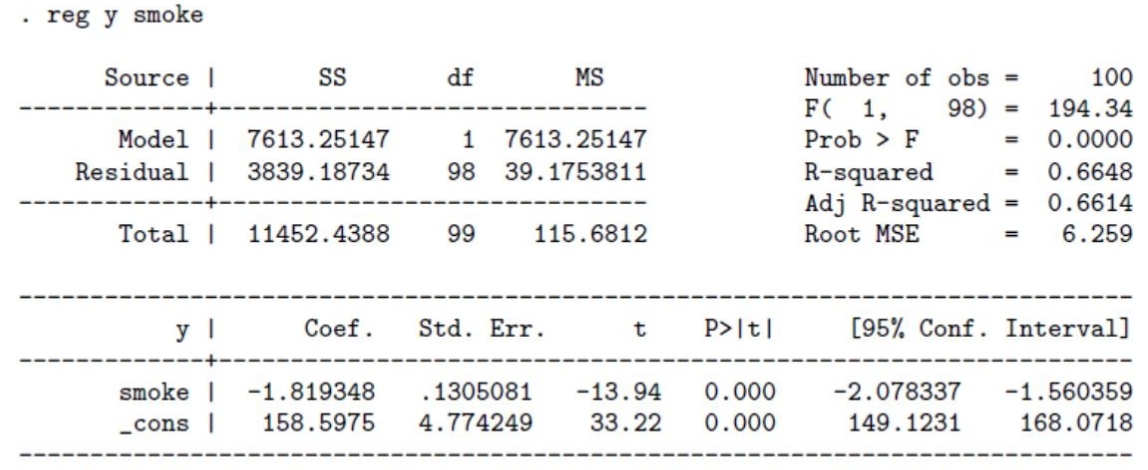
\includegraphics[width=0.8\linewidth]{../Imagenes/RegySmoke.jpeg}
    \end{figure}
    \begin{itemize}
        \item $\hat{\tilde{\beta}}_{1}=-1.81$
        \item ¿Qué variables estamos omitiendo aca?
    \end{itemize}
\end{frame}

\begin{frame}{Ejemplo 2}
    \begin{itemize}
        \item ¿Y si agregamos edad?
        \begin{figure}
            \centering
            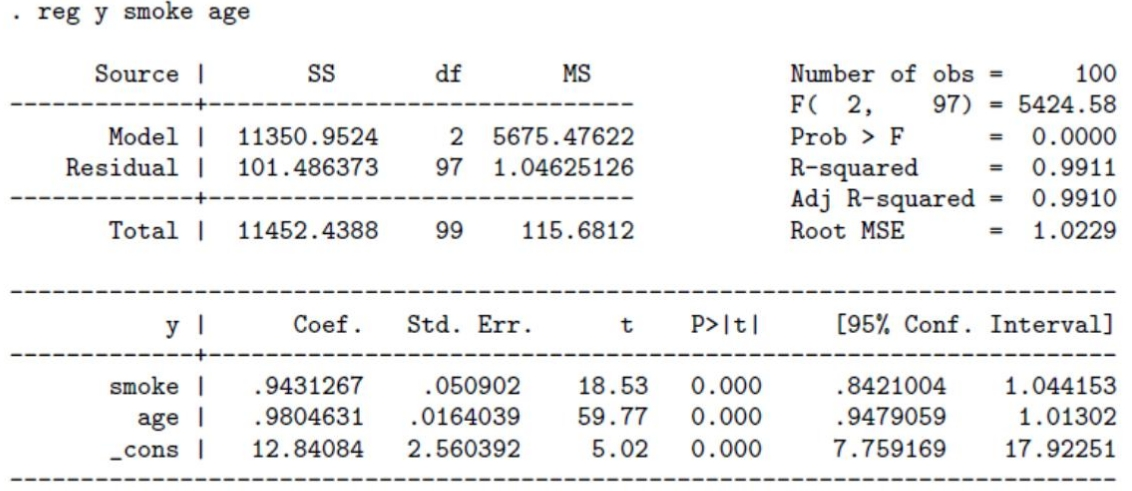
\includegraphics[width=0.8\linewidth]{../Imagenes/RegySmokeAge.jpeg}
        \end{figure}
    \end{itemize}
    \begin{itemize}
        \item Si este fuera el modelo verdadero, $\hat{\beta}_{1}=0.94>\hat{\tilde{\beta}}_{1}=-1.81$. Si $\hat{\beta}_{2}>0$, ¿qué me dice esto sobre el signo de relaci\'on entre edad y fumar cigarrillos $\delta_{2}$?
        \item Recuerden: $\tilde{\beta}_{1}=\beta_{1}+\beta_{2} \delta_{2}$
        \item Es negativa: cuanto mayor es la persona, menos fuma.
    \end{itemize}
\end{frame}

\begin{frame}{¿Más es mejor?}
    \begin{itemize}
        \item Uno podría pensar que tiene que agregar todas las variables posibles al modelo, para evitar omitir variables.
        \item Sin embargo, esto trae problemas.
        \item Se dice que un modelo está sobreespecificado cuando se incluye en la regresión variables que no forman parte del modelo poblacional.
        \item Incluir variables irrelevantes en el modelo no influye en el insesgamiento de los estimadores, pero  incrementa la varianza de los estimadores.
    \end{itemize}
\end{frame}

\begin{frame}{Sin sesgo de selección}
    \begin{itemize}
        \item Si tenemos la suerte de tener una aleatorización que nos garantiza que no haya sesgo de selección, ¿importa agregar variables adicionales?
        \item Si $X_{1}$ (o $T_{i}$ en t\'erminos de tratamiento) se determina de forma aleatoria, nos garantiza que $E\left[\epsilon_{i} \mid X_{i}\right]=0$
        \item ¡La correlaci\'on entre cualquier variable no incluida en el modelo y el tratamiento será 0!
        \item Entonces, no necesitamos incluir otras variables en el modelo para evitar sesgos.
      
    \end{itemize}
\end{frame}

\begin{frame}{Conclusiones}
    \begin{itemize}
        \item Incluir variables a un modelo cambia la interpretación de nuestra variable de interés.
        \item El impacto de la exclusión de una variable relevante depende de la correlación entre la variable de interés y la variable omitida y la relación entre la variable omitida y el outcome.
        \item El supuesto clave de MCO para que no haya sesgo es que $E[\epsilon \mid X]=0$.
               \item Es poco frequente que tengamos TODAS las variables que determinan la asignación y entonces, es poco probable que la inclusión de variables nos permita dar una interpretación causal a una regresión lineal.
    \end{itemize}
\end{frame}

\begin{frame}{Ejercicio final}
    \begin{itemize}
        \item Queremos estimar el efecto causal de asistir a preuniversitario sobre el puntaje PSU:
        $$
        puntaje_i=\alpha+\beta_1 preu_i+u_i
        $$
        donde $preu_i=1$ si el estudiante asistió a preuniversitario.
        \item La variable omitida es el apoyo familiar, $apoyo_i$, que afecta el puntaje y también la probabilidad de asistir a preuniversitario.
        \item Suponga que el modelo verdadero es:
        $$
        puntaje_i=\alpha+\beta_1 preu_i+\beta_2 apoyo_i+u_i
        $$
        y que:
        $$
        apoyo_i=\delta_0+\delta_1 preu_i+v_i
        $$
        \item Si $\beta_1=25$, $\beta_2=40$ y $\delta_1=0{,}5$, responda:
        \begin{enumerate}
            \item ¿Cuál es el sesgo por variable omitida?
            \item ¿Cuál será el coeficiente estimado al omitir $apoyo_i$?
            \item ¿Se sobreestima o subestima el efecto causal del preuniversitario?
        \end{enumerate}
    \end{itemize}
\end{frame}

\begin{frame}{Solución ejercicio final}
    \begin{itemize}
        \item La fórmula del coeficiente estimado cuando omitimos $apoyo_i$ es:
        $$
        \tilde{\beta}_{1}=\beta_1+\beta_2\delta_1
        $$
        \item Entonces, el sesgo es:
        $$
        \beta_2\delta_1=40\cdot 0{,}5=20
        $$
        \item Por lo tanto:
        $$
        \tilde{\beta}_{1}=25+20=45
        $$
        \item La regresión simple estimaría que asistir a preuniversitario aumenta el puntaje en 45 puntos.
        \item Pero el efecto causal verdadero era 25 puntos. Entonces, el efecto está \textbf{sobreestimado}.
        \item Intuición: estudiantes con más apoyo familiar tienden a asistir más al preuniversitario y, además, ese apoyo aumenta su puntaje. Al omitirlo, parte del efecto del apoyo familiar se atribuye erróneamente al preuniversitario.
    \end{itemize}
\end{frame}



\end{document}
